% Options for packages loaded elsewhere
\PassOptionsToPackage{unicode}{hyperref}
\PassOptionsToPackage{hyphens}{url}
%
\documentclass[
  8pt,
  ignorenonframetext,
]{beamer}
\usepackage{pgfpages}
\setbeamertemplate{caption}[numbered]
\setbeamertemplate{caption label separator}{: }
\setbeamercolor{caption name}{fg=normal text.fg}
\beamertemplatenavigationsymbolsempty
% Prevent slide breaks in the middle of a paragraph
\widowpenalties 1 10000
\raggedbottom
\setbeamertemplate{part page}{
  \centering
  \begin{beamercolorbox}[sep=16pt,center]{part title}
    \usebeamerfont{part title}\insertpart\par
  \end{beamercolorbox}
}
\setbeamertemplate{section page}{
  \centering
  \begin{beamercolorbox}[sep=12pt,center]{part title}
    \usebeamerfont{section title}\insertsection\par
  \end{beamercolorbox}
}
\setbeamertemplate{subsection page}{
  \centering
  \begin{beamercolorbox}[sep=8pt,center]{part title}
    \usebeamerfont{subsection title}\insertsubsection\par
  \end{beamercolorbox}
}
\AtBeginPart{
  \frame{\partpage}
}
\AtBeginSection{
  \ifbibliography
  \else
    \frame{\sectionpage}
  \fi
}
\AtBeginSubsection{
  \frame{\subsectionpage}
}
\usepackage{amsmath,amssymb}
\usepackage{lmodern}
\usepackage{iftex}
\ifPDFTeX
  \usepackage[T1]{fontenc}
  \usepackage[utf8]{inputenc}
  \usepackage{textcomp} % provide euro and other symbols
\else % if luatex or xetex
  \usepackage{unicode-math}
  \defaultfontfeatures{Scale=MatchLowercase}
  \defaultfontfeatures[\rmfamily]{Ligatures=TeX,Scale=1}
\fi
\usetheme[]{Berkeley}
% Use upquote if available, for straight quotes in verbatim environments
\IfFileExists{upquote.sty}{\usepackage{upquote}}{}
\IfFileExists{microtype.sty}{% use microtype if available
  \usepackage[]{microtype}
  \UseMicrotypeSet[protrusion]{basicmath} % disable protrusion for tt fonts
}{}
\makeatletter
\@ifundefined{KOMAClassName}{% if non-KOMA class
  \IfFileExists{parskip.sty}{%
    \usepackage{parskip}
  }{% else
    \setlength{\parindent}{0pt}
    \setlength{\parskip}{6pt plus 2pt minus 1pt}}
}{% if KOMA class
  \KOMAoptions{parskip=half}}
\makeatother
\usepackage{xcolor}
\newif\ifbibliography
\setlength{\emergencystretch}{3em} % prevent overfull lines
\providecommand{\tightlist}{%
  \setlength{\itemsep}{0pt}\setlength{\parskip}{0pt}}
\setcounter{secnumdepth}{-\maxdimen} % remove section numbering
\AtBeginSubsection{}
\AtBeginSection{}
\ifLuaTeX
  \usepackage{selnolig}  % disable illegal ligatures
\fi
\IfFileExists{bookmark.sty}{\usepackage{bookmark}}{\usepackage{hyperref}}
\IfFileExists{xurl.sty}{\usepackage{xurl}}{} % add URL line breaks if available
\urlstyle{same} % disable monospaced font for URLs
\hypersetup{
  pdftitle={Using people-like-me method to study the children height growth with EPIC data},
  pdfauthor={Randy},
  hidelinks,
  pdfcreator={LaTeX via pandoc}}

\title{Using people-like-me method to study the children height growth
with EPIC data}
\subtitle{An extension for predictive mean matching with Mahalanobis
distrance}
\author{Randy}
\date{}
\institute{Department of Biostatistics \& Informatics}

\begin{document}
\frame{\titlepage}

\begin{frame}[allowframebreaks]
  \tableofcontents[hideallsubsections]
\end{frame}
\hypertarget{background}{%
\section{Background}\label{background}}

\begin{frame}{Data}
\protect\hypertarget{data}{}
The EPIC Observational Study:

\begin{itemize}
\tightlist
\item
  Prospective, multi-center, observational longitudinal study
\item
  Collected through the Cystic Fibrosis Foundation Patient Registry
  (CFFPR)
\item
  Of the 1772 children enrolled, we identified \textbf{1325 individuals}
  with usable data, total 76497 visit observations
\end{itemize}

For this study,

\begin{itemize}
\tightlist
\item
  913 children are randomly assigned as training group
\item
  The other 457 children are assigned as testing group
\end{itemize}
\end{frame}

\begin{frame}{Data}
\protect\hypertarget{data-1}{}
\begin{center}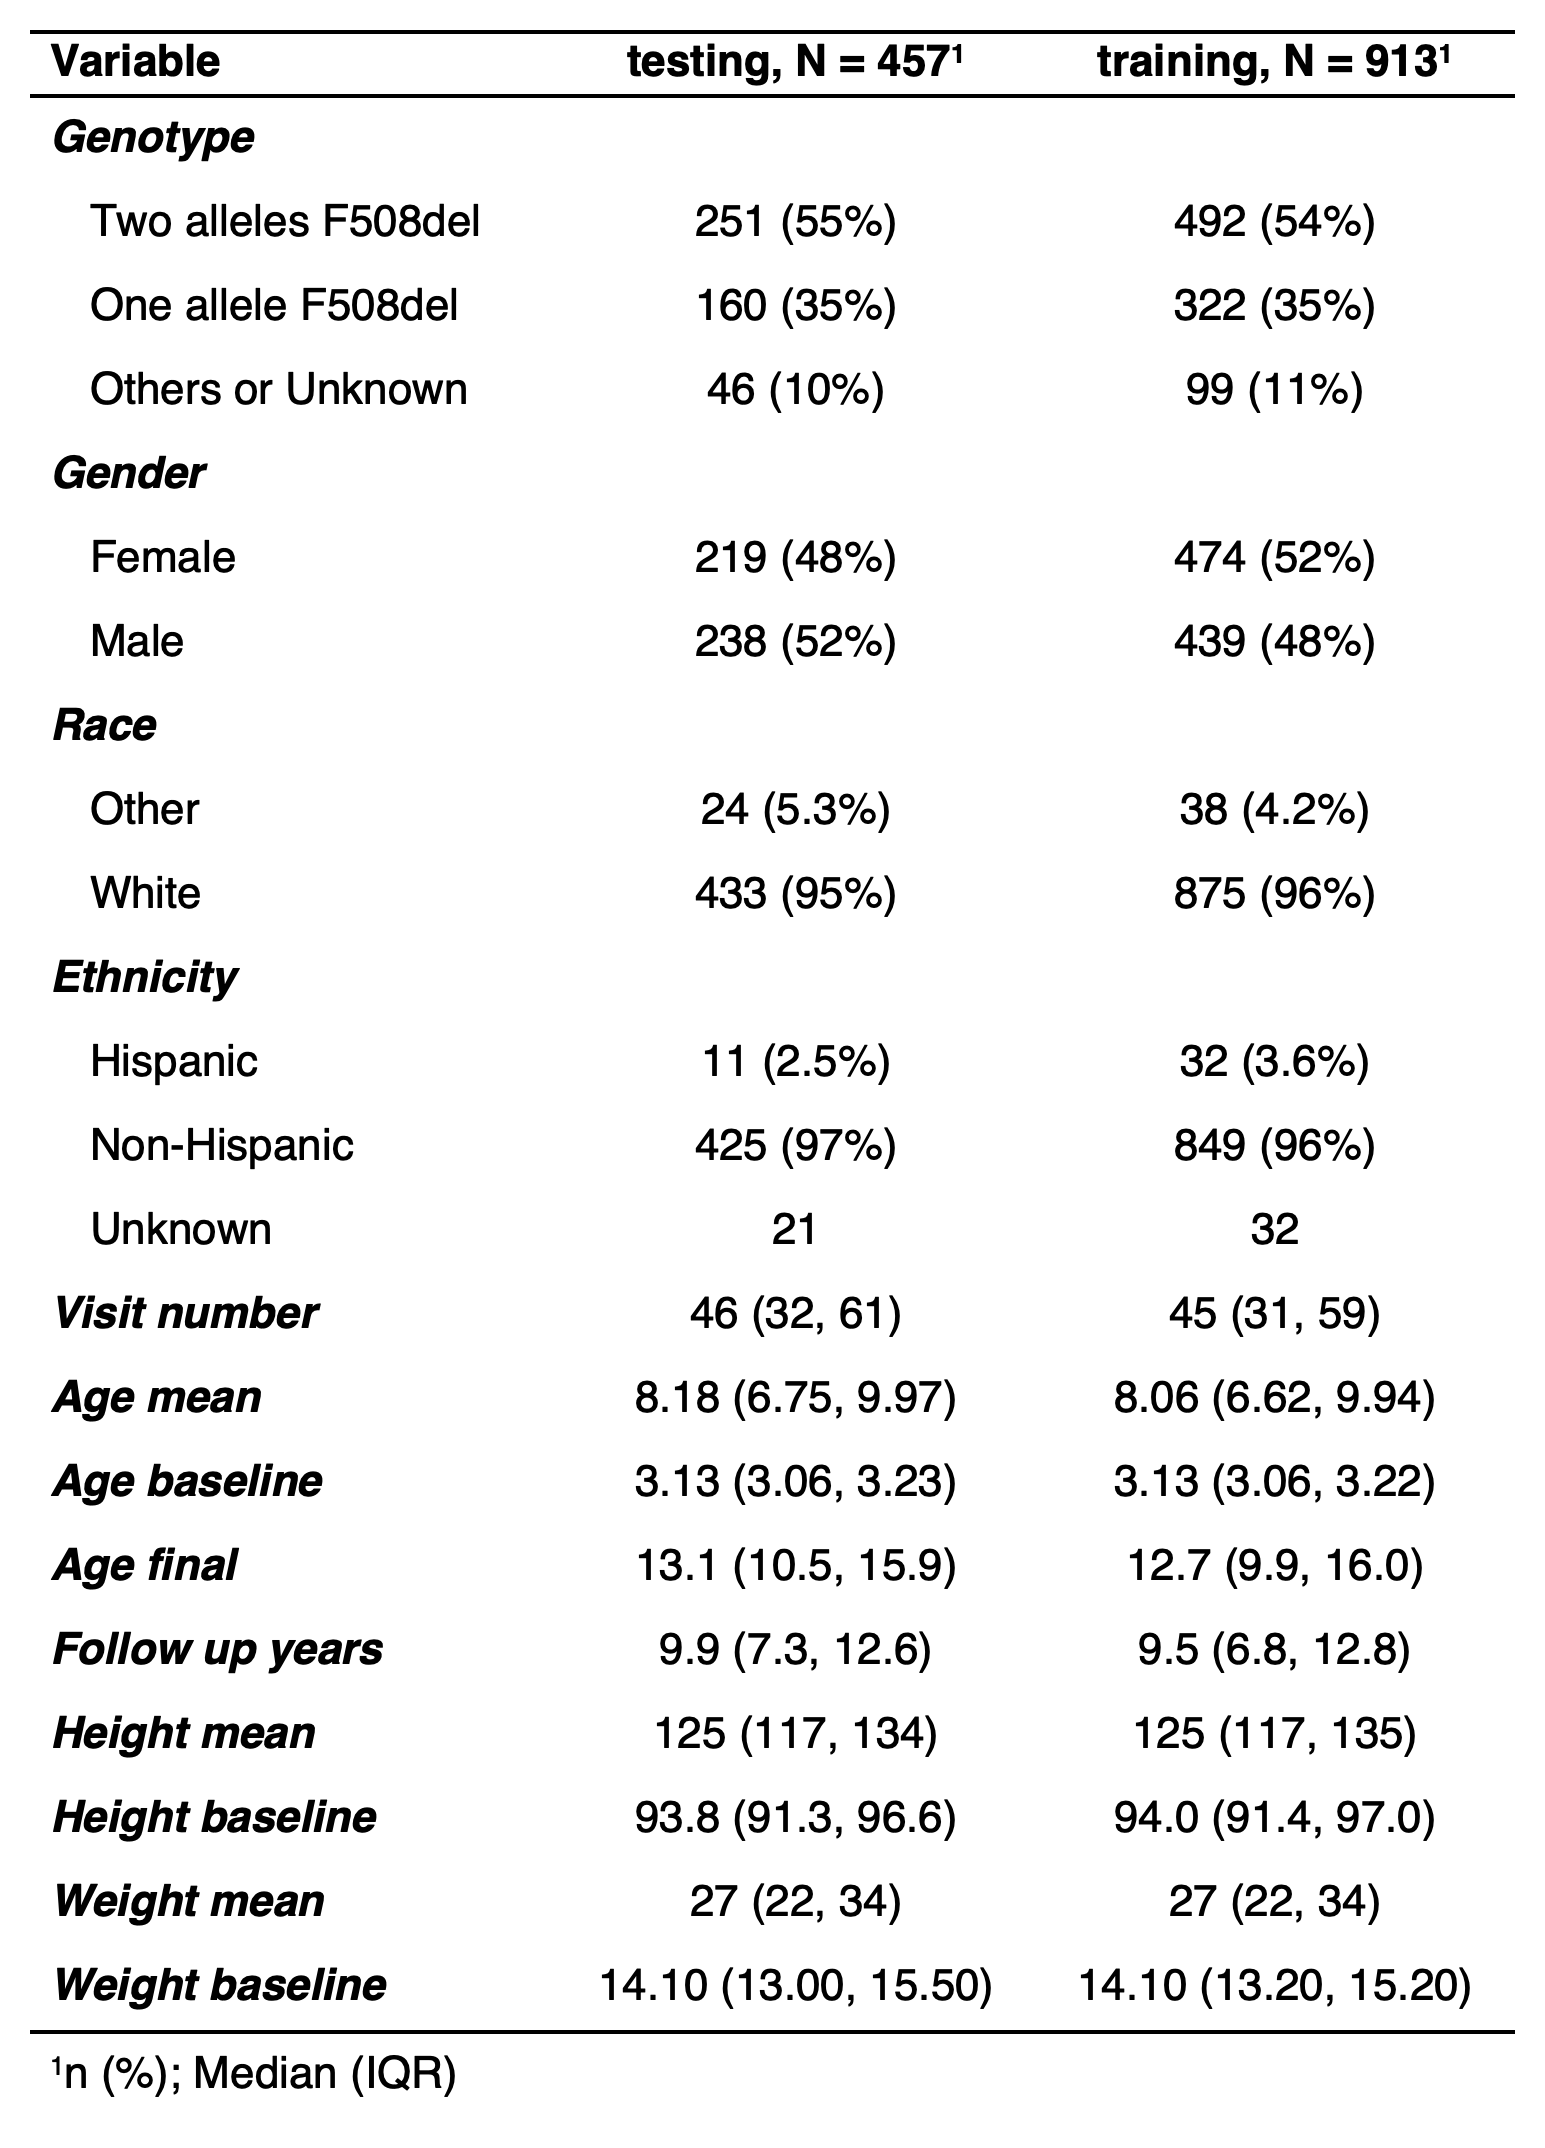
\includegraphics[width=0.5\linewidth]{figure/01_table1} \end{center}
\end{frame}

\begin{frame}{People-like-me}
\protect\hypertarget{people-like-me}{}
The traditional predictive modeling:

\begin{itemize}
\tightlist
\item
  A global inference and universal modelling over all available data.
\item
  Overlooking the cultural diversity and genetic heterogeneity for
  patients
\end{itemize}

People-like-me method:

\begin{itemize}
\tightlist
\item
  Individualized curving matching
\item
  To use fewer but more similar samples
\item
  To get a higher predictive performance than with more similar matches
\item
  Information of \textbf{\emph{the nearest neighbors of predictive
  mean}}
\end{itemize}
\end{frame}

\begin{frame}{Predictive mean matching}
\protect\hypertarget{predictive-mean-matching}{}
\begin{itemize}
\tightlist
\item
  The imputations created by predictive mean matching follow the data
  nicely
\item
  With respect to \textbf{certain metrics}
\item
  To avoid the dataset noise and model misspecification
\end{itemize}

\textbf{Through exhaustive comparisons with predictive mean, for
specific target and the most similar matching donor-cohort}
\end{frame}

\begin{frame}{Donor-cohort}
\protect\hypertarget{donor-cohort}{}
\begin{enumerate}
\tightlist
\item
  ``The chosen threshold''
\end{enumerate}

Choose a threshold, and take all donors agreed within this threshold

\begin{enumerate}
\setcounter{enumi}{1}
\tightlist
\item
  ``The nearest neighbor''
\end{enumerate}

Decide the number of matching donors, and choose this number of donors
with minimal metrics.

\begin{enumerate}
\setcounter{enumi}{2}
\item
  ``Single-time'' v.s ``Multiple-time''
\item
  Which metric to use
\end{enumerate}

In the past: with predictive mean matching with \emph{single time point}
and a \emph{fixed} number of candidate donors.
\end{frame}

\begin{frame}{Example}
\protect\hypertarget{example}{}
\begin{figure}

{\centering 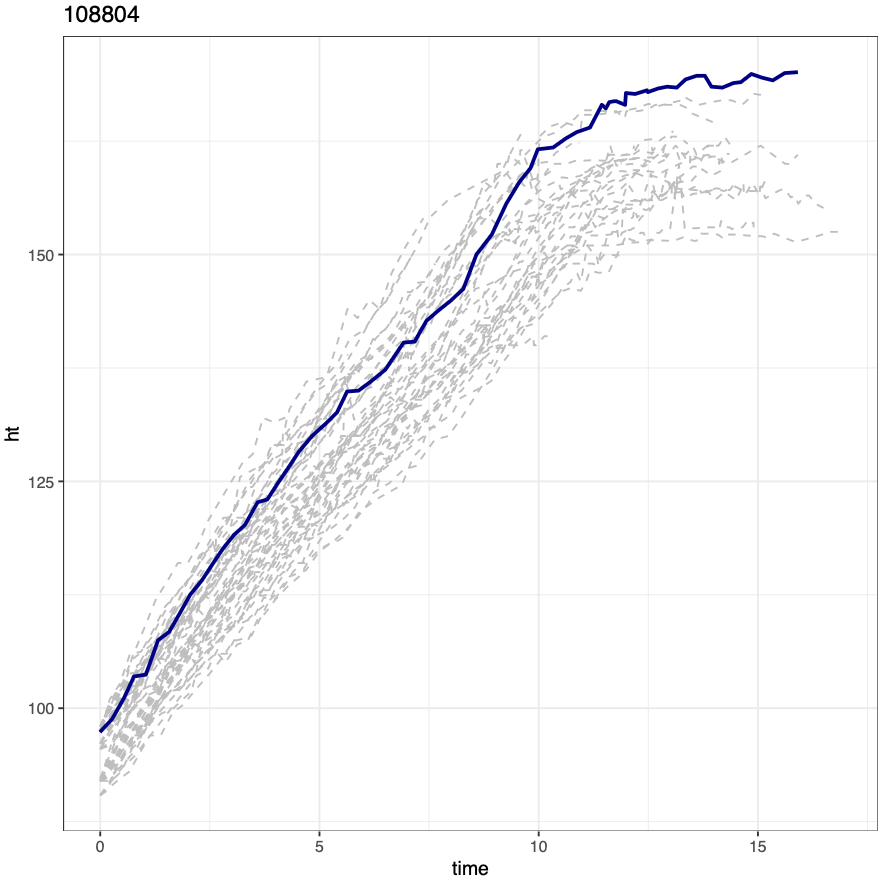
\includegraphics[width=0.4\linewidth]{figure/fig01} 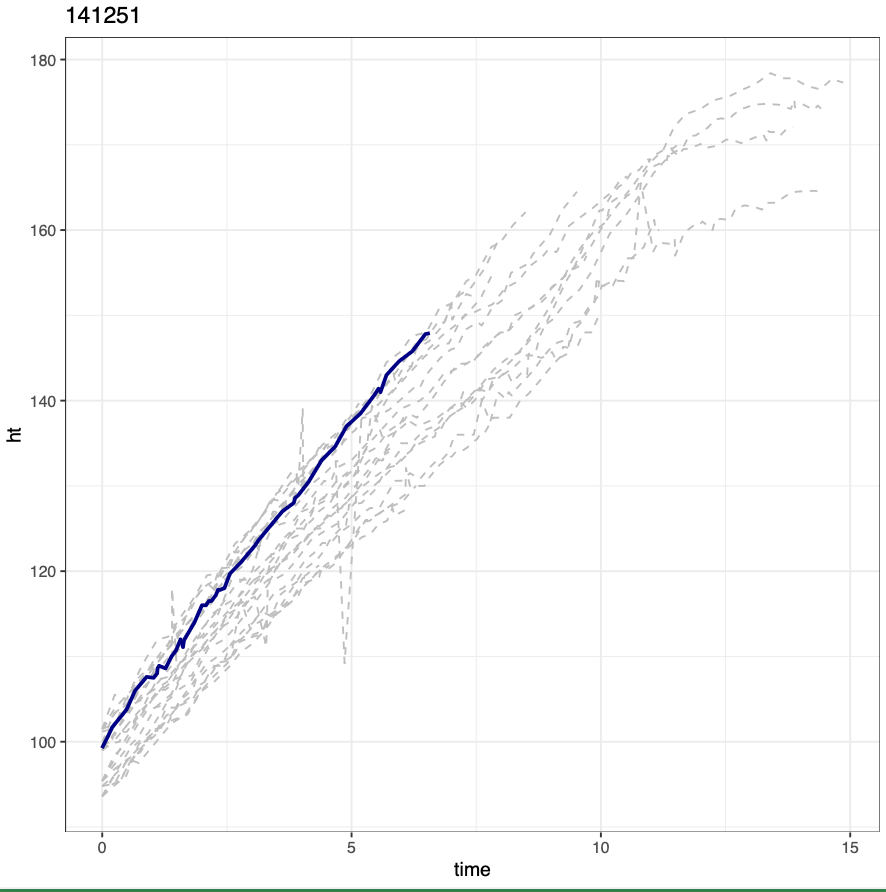
\includegraphics[width=0.4\linewidth]{figure/fig02} 

}

\caption{Individual matching trajectoreis example}\label{fig:Example trajectories for sample matching}
\end{figure}
\end{frame}

\begin{frame}{Mahalanobis Distance}
\protect\hypertarget{mahalanobis-distance}{}
\begin{itemize}
\tightlist
\item
  Mahalanobis distance is a multivariate distance metric, measuring the
  distance between a point and a distribution.
\end{itemize}

\[
\pmb D^2 = (\pmb x - \pmb \mu)^T \cdot \pmb \Sigma^{-1} \cdot (\pmb x - \pmb \mu)
\]

Where:

\begin{itemize}
\item
  \(\pmb D^2\) is the square of the Mahalanobis distance
\item
  \(\pmb x\) is the vector of the observation (\(n\) row in a dataset)
\item
  \(\pmb \mu\) is the vector of mean values of independent variables
  (mean of each column)
\item
  \(\pmb \Sigma\) is the covariance matrix of independent variables.
\item
  The squared Mahalanobis distance, \(\pmb D^2\), is Chi-square
  distributed.
\item
  Based on the \(\chi^2\) test \(p\)-value, we can find the acceptance
  of given donors.
\end{itemize}
\end{frame}

\hypertarget{what-we-got-so-far}{%
\section{What we got so far}\label{what-we-got-so-far}}

\begin{frame}[fragile]{Steps}
\protect\hypertarget{steps}{}
\begin{itemize}
\tightlist
\item
  Fitting a \texttt{brokenstick} model with training dataset and getting
  the predictive imputations
\end{itemize}

\begin{verbatim}
brokenstick_prediction(formula = "ht ~ time | id",
                       train_data = train,
                       knots = c(5, 10, 12),
                       pred_time = c(2, 4, 6, 8, 10, 12, 14),
                       newdata = test_baseline)
\end{verbatim}

\begin{itemize}
\tightlist
\item
  Fitting a \texttt{linear\ model} at for all the subjects with baseline
  information
\item
  Getting the predictive values at each time point from
  \texttt{linear\ models}
\end{itemize}

\begin{verbatim}
linearized_brokenstick(lm_formula = "`.pred` ~ time_factor * sex + baseline + ...",
                      bks_pred = bks_pred)
\end{verbatim}
\end{frame}

\begin{frame}[fragile]{Steps}
\protect\hypertarget{steps-1}{}
With each subject from testing dataset,

\begin{itemize}
\tightlist
\item
  Calculating the metrics, e.g.~Euclidean distance or Mahalanobis
  distance, between the target with all the others in training dataset
\item
  Deciding on the set and the size of \texttt{donor-cohort}
\item
  Fitting \texttt{gamlss} model with \texttt{donor-cohort} observations
\item
  Getting the prediction and confidence intervals
\end{itemize}

\begin{verbatim}
pred_matching(lb_data = lb_data, obs_data = test_data,
              match_methods = c("mahalanobis", "euclidean", "singletime"),
              match_alpha or match_number,
              gamlss_formula = "ht ~ cs(time, df = 3)",  
              gamsigma_formula = "~ cs(time, df = 1)",
              match_plot = TRUE,  predict_plot = TRUE,)
\end{verbatim}
\end{frame}

\begin{frame}{Simulation of 20 datasets}
\protect\hypertarget{simulation-of-20-datasets}{}
\begin{center}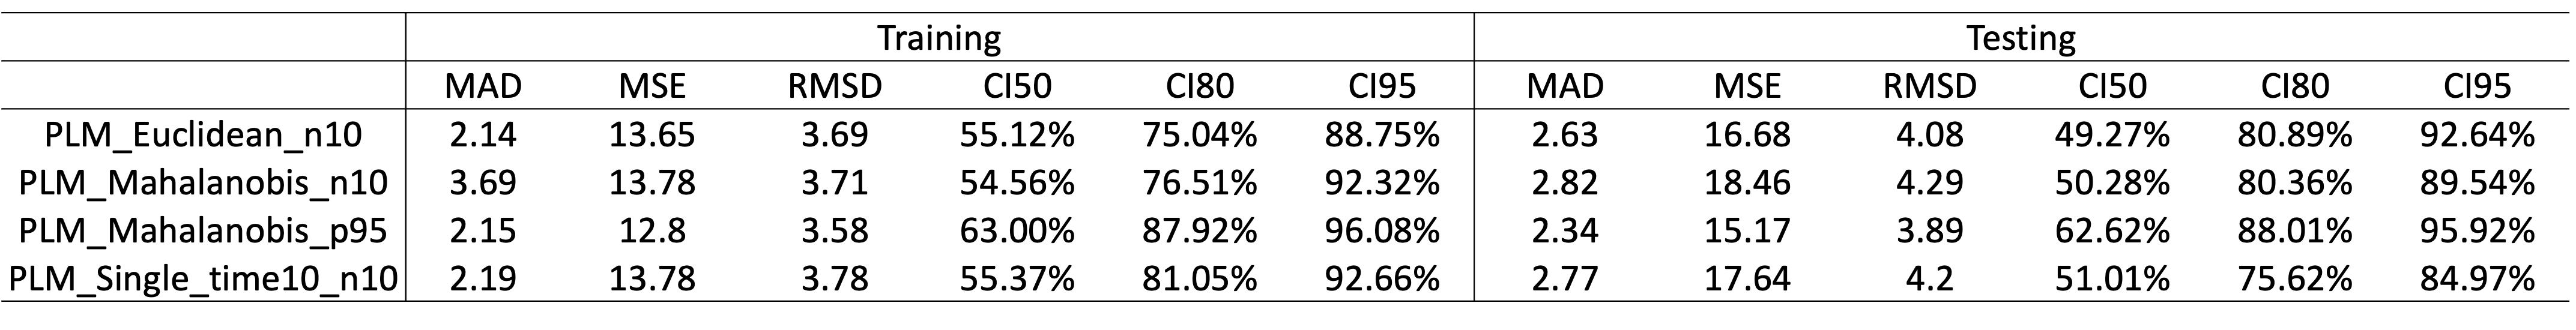
\includegraphics[width=1.2\linewidth]{figure/fig3} \end{center}

A larger simulation study with 1000 datasets is going on with
\href{https://www.osgconnect.net/}{OGS Connect}
\end{frame}

\begin{frame}{Large Simulation Study with 1000 datasets}
\protect\hypertarget{large-simulation-study-with-1000-datasets}{}
Bias

\begin{center}\includegraphics[width=1\linewidth]{test_bias_simulation_20221020} \end{center}
\end{frame}

\begin{frame}{}
\protect\hypertarget{section}{}
RMSE

\begin{center}\includegraphics[width=1\linewidth]{test_rmse_simulation_20221020} \end{center}
\end{frame}

\begin{frame}{}
\protect\hypertarget{section-1}{}
Coverage50

\begin{center}\includegraphics[width=1\linewidth]{test_coverage50_simulation_20221020} \end{center}
\end{frame}

\begin{frame}{Coverage80}
\protect\hypertarget{coverage80}{}
\begin{center}\includegraphics[width=1\linewidth]{test_coverage80_simulation_20221020} \end{center}
\end{frame}

\begin{frame}{Coverage90}
\protect\hypertarget{coverage90}{}
\begin{center}\includegraphics[width=1\linewidth]{test_coverage90_simulation_20221020} \end{center}
\end{frame}

\begin{frame}[fragile]{Package and Shinyapp}
\protect\hypertarget{package-and-shinyapp}{}
\begin{verbatim}
library(plmlmm)

plmlmm::run_shiny()
\end{verbatim}
\end{frame}

\hypertarget{paper}{%
\section{Paper}\label{paper}}

\begin{frame}{Paper}
\begin{itemize}
\item
  Finish the data analysis and simulation study
\item
  Abstract
\item
  Introduction (**)
\item
  Dataset Epic (in detals)

  \begin{itemize}
  \item
    table1 (**)
  \item
    sample trajectory (**)
  \end{itemize}
\item
  Methods

  \begin{itemize}
  \tightlist
  \item
    People-like-me methods

    \begin{itemize}
    \tightlist
    \item
      Euclidean distance v.s. Mahalanobis distance
    \item
      Single time v.s. Multiple time
    \item
      fixed sample size v.s. unfixed sample size
    \end{itemize}
  \item
    Dynamic prediction
  \end{itemize}
\item
  Results

  \begin{itemize}
  \tightlist
  \item
    Analysis for Epic data

    \begin{itemize}
    \tightlist
    \item
      different setting
    \item
      results summary
    \end{itemize}
  \item
    Simulation study 1000 dataset
  \end{itemize}
\item
  Discussion and Extension

  \begin{itemize}
  \tightlist
  \item
    use a Guassian kernel for Mahalanobis distance
  \item
    parameter tuning why use \(\alpha = 0.9\)
  \end{itemize}
\end{itemize}
\end{frame}

\end{document}
